\begin{frame}{Key Observation}

\begin{block}{Lemma 1 (informal)}
SGD satisfies
\begin{equation}
\text{generalization error} = O\left( \frac{\lF{\nabla \ell}}{\sqrt n} \right)
\end{equation}
\end{block}

\begin{itemize}
\item
Immediate corrollary of standard properties of SGD

\citep{shalev2014understanding}

\vspace{0.2in}
\uncover<2->{
\item
Painful notation to formalize this
}

        \uncover<4->{
\vspace{0.2in}
\item Recover known bounds:
\begin{equation*}
\lF{\nabla\ell} = \lF{W^*} = O(\sqrt{kd})
\quad\Rightarrow
\text{generalization error} = O(\sqrt{kd/n})
\end{equation*}
}

%(IMNSO: most important skill for new mathematician to learn

\uncover<5>{
%\vspace{0.2in}
\item \textbf{Idea:} 
Rewrite the cross entropy loss so that $\lF{\nabla\ell}$ is smaller
\begin{itemize}
\vspace{0.1in}
\item For people familiar with the notation, this change is ``trivial''
\end{itemize}
}
\end{itemize}

\uncover<3> {
    \begin{center}
    \vspace{-3.45in}
    \setlength{\fboxsep}{0pt}%
    \setlength{\fboxrule}{1pt}%
    \fbox{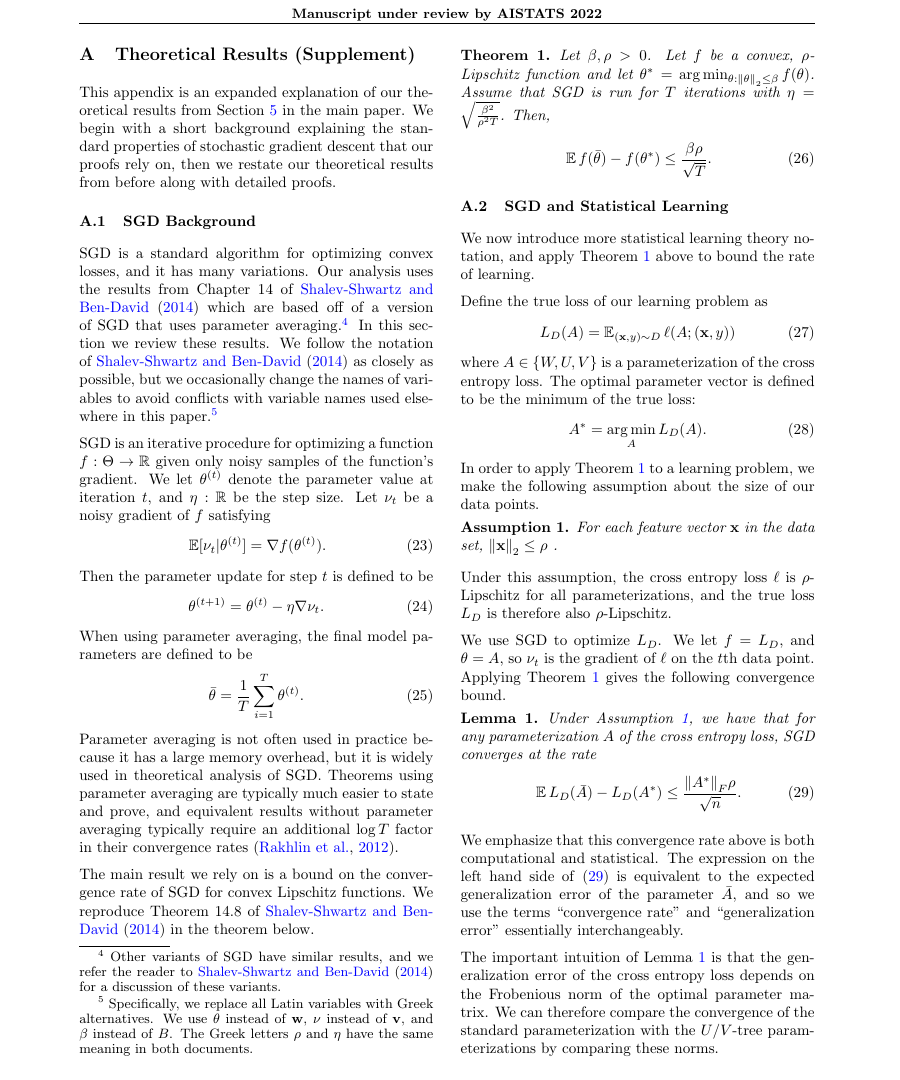
\includegraphics[height=3.5in]{img/lemma1-paper}}
    \end{center}
}
\uncover<5> {~}

\end{frame}

%%%%%%%%%%%%%%%%%%%%%%%%%%%%%%%%%%%%%%%%%%%%%%%%%%%%%%%%%%%%%%%%%%%%%%%%%%%%%%%%

%\begin{frame}{Key Ideas}
%\begin{block}{Lemma 1 (informal)}
%\begin{equation}
%\text{generalization error} \le \frac{\beta\rho}
%\end{equation}
%\end{block}
%\end{frame}


